\documentclass[a4paper]{article}

\usepackage{amsmath}
\usepackage{enumitem}

\usepackage{subfigure}
\usepackage{amsmath}
\usepackage{amssymb}
\usepackage{graphicx}

\usepackage[font=small,labelfont=bf]{caption}

\DeclareMathOperator*{\argmin}{arg\,min}
\author{Kennard Ng and Luo Wen Han}
\title{Project 2: Latent Dirichlet Allocation}

\bibliographystyle{unsrt}

\begin{document}
	\maketitle
	\section{Introduction}
	
	% todo: add motivatin
	
	In this report, we make inferences on the ancestry of individuals given their genotype. More specifically, we model the relationship between a person's genotype and his ancestors using the Latent Dirchlet Allocation (LDA) model~\cite{blei2003latent} and use variational inference to discover the ancestor populations' of individuals. 

	\section{Background}
	
	\subsection{Notations and Terminology}
	
	In our problem, we define the following:
	\begin{itemize}[noitemsep]
		\item a genotype $w \in \{w^v\}_{1:V}$ is an atomic unit in genetics where each genotype is represented as a one-hot encoded vector of length $V$ where $V$ is the number of genotypes. 
		\item an individual is represented as a sequence of $N$ genotypes $\mathbf{w} = \{w_n\}_{1:N}$.
	\end{itemize}
	
	
	\subsection{Latent Dirichlet Distribution}
	
	Intuitively, each individual's sequence of genotypes are inherited from his ancestors where under the generative probabilitistic model of LDA model, individuals can be represented as random mixtures over latent ancestor populations, where each ancestor population can be described by a distribution over genotypes. More specifically, the generative process for each individual is the following: 
	
	\begin{enumerate}[noitemsep]
		\item Choose $\theta \sim \mathrm{Dir}(\alpha)$.
		\item For each of the $N$ genotypes $w_n$:
		\begin{enumerate}[noitemsep]
			\item Choose an ancestor population $z_n \sim \mathrm{Multinomial}(\theta)$.
			\item Choose a genotype $w_n$ from $p(w_n|z_n,\beta)$, where $p(w_n|z_n,\beta)$ is a multinomial distribution conditioned on the ancestor population $z_n$ and $\beta$,
		\end{enumerate}
	\end{enumerate}
	\noindent where $\beta$ is $k \times V$ matrix of genotype probabilities conditioned on topic $z \in \{z_k\}_{1:K}$ i.e. $\beta_{ij} = p(w^i|z_j)$ and $\alpha$ $k$-vector parameter with components $\alpha_i > 0$ such that:
	\begin{equation}
		p(\mathbf{\theta} \mid \mathbf{\alpha}) = \frac{\Gamma\left(\sum_{i=1}^{k} \alpha_{i}\right)}{\prod_{i=1}^{k} \Gamma\left(\alpha_{i}\right)} \theta_{1}^{\alpha_{1}-1} \cdots \theta_{k}^{\alpha_{k}-1},
	\end{equation}
	\noindent where $\gamma(\cdot)$ is the Gamma function. The graphical model representation of the LDA model is given in Figure~\ref{fig:ldagraphical}.
	
	
	\begin{figure}[ht]
		\centering
		\captionsetup{width=.8\linewidth}
		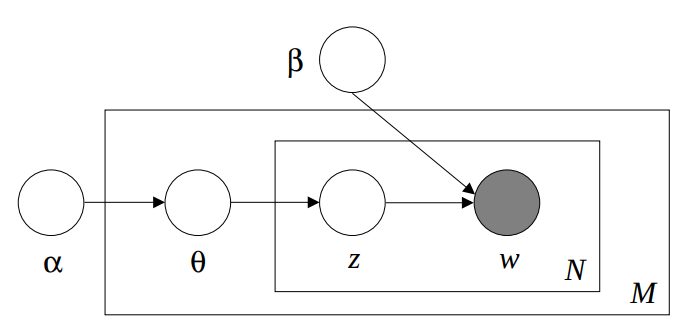
\includegraphics[width=0.6\linewidth]{images/lda_graphical}
		\caption{Graphical Model of LDA. Taken from~\cite{blei2003latent}. The plates represent replicas. In our context, the inner plate represents the repeated choice of ancestor populations and genotypes of a person while the outer plate represents the population with $M$ individuals. Notice also that by observing $w$, $\beta$ and $\theta$ are coupled together (head-to-head relationship).}
		\label{fig:ldagraphical}
	\end{figure}

	\subsection{Variational Inference}
	
	During inference, we want to find the posterior distributions over hidden variables $\theta, \mathbf{z}$ given parameters $\alpha, \beta$ and observed variables $\mathbf{w}$. We express this as the following posterior distribution:
	
	\begin{equation}
		p(\theta, \mathbf{z} | \mathbf{w}, \alpha, \beta)=\frac{p(\theta, \mathbf{z}, \mathbf{w} | \alpha, \beta)}{p(\mathbf{w} | \alpha, \beta)}.
	\end{equation}
	
	\noindent Unfortunately, we see that exact inference is intractable given that the normalizer is intractable where marginalizing over the hidden variables gives:
	\begin{equation}
	\begin{aligned}
	p(\mathbf{w} | \alpha, \beta)&=\int p(\theta | \alpha)\left(\prod_{n=1}^{N} \sum_{z_{n}} p\left(z_{n} | \theta\right) p\left(w_{n} | z_{n}, \beta\right)\right) d \theta\\
	&=\frac{\Gamma\left(\Sigma_{i} \alpha_{i}\right)}{\prod_{i} \Gamma\left(\alpha_{i}\right)} \int\left(\prod_{i=1}^{k} \theta_{i}^{\alpha_{i}-1}\right)\left(\prod_{n=1}^{N} \sum_{i=1}^{k} \prod_{j=1}^{V}\left(\theta_{i} \beta_{i j}\right)^{w_{n}^{j}}\right) d \theta,
	\end{aligned}
	\end{equation}
	\noindent which is intractable due to the coupling between $\beta$ and $\theta$. Hence, we instead use approximate inference where, under the Mean Field assumption, we remove the problematic edges between $\theta, \mathbf{z}$ and $\mathbf{w}$, the node $\mathbf{w}$ and endow our model with free variational parameters, introducing the following variational distribution:
	\begin{equation}
		q(\theta,z \mid \gamma,\phi) = q(\theta\mid\gamma) \prod_{n=1}^{N} q(z_n\mid\phi_n).
	\end{equation}
	
	\noindent where the Dirchlet parameter $\gamma$ and the multinomial parameters $\left\{\phi_n\right\}_{1:N}$ are free variational parameters. The graphical model representation of the variationl distribution based on the mean field assumption is given in Figure~\ref{fig:approximategraphical}.
	
	\begin{figure}[ht]
		\centering
		\captionsetup{width=.8\linewidth}
		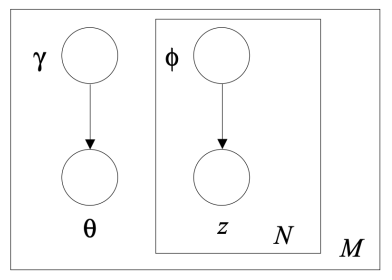
\includegraphics[width=0.5\linewidth]{images/approximate_graphical}
		\caption{Approximate Distribution under the Mean Field Assumption.}
		\label{fig:approximategraphical}
	\end{figure}
	
	 Blei et al.~\cite{blei2003latent} show that the optimal values of the variational parameters $\gamma$ and $\phi$ can be computed by minimizing the Kullback-Leibler (KL) divergence between the approximate distribution and the true posterior where:
	\begin{equation}
		(\gamma^*,\phi^*) = \argmin_{(\gamma,\phi)} \mathbf{KL}(q(\theta,\mathbf{z} \mid \gamma, \phi) \parallel p(\theta,\mathbf{z} \mid \mathbf{w},\alpha,\beta))
	\end{equation}
	
	\noindent We minimize the KL-divergence via an iterative fixed-point method using the following update equations dervied by taking the derivatives of the KL divergence w.r.t. the variational parameters and setting them to zero: 
	\begin{equation}
		\phi_{ni} \propto \beta_{iw_n} \exp\left\{\mathbb{E}_q\left[\log{(\theta_i)}  \mid \gamma\right]\right\},
		\label{eqn:e_step}
	\end{equation}
	\begin{equation}
		\gamma_i = \alpha_i + \textstyle \sum_{n=1}^N \phi_{ni},
		\label{eqn:m_step}
	\end{equation}
	where the expectation in the multinomial update in~\ref{eqn:e_step} can be computed by: 
	\begin{equation}
	\mathbb{E}_q\left[\log{(\theta_i)}  \mid \gamma \right] = \Psi(\gamma_i)-\Psi\left(\sum_{j=1}^k \gamma_j\right)
	\label{eqn:expectation}
	\end{equation}
	where $\Psi$ is the first derivative of the $\log\Gamma$ function computed from Taylor approximation. The iterative fixed point method is summarized to be following:
	\begin{enumerate}[noitemsep]
		\item $\forall i,n, \quad \phi^0_{ni} = 1/k$ and $\forall i, \quad \gamma_i = \alpha_i + N / k$.
		\item repeat until convergence: 
		\begin{enumerate}[noitemsep]
			\item for $n \in \{1, \cdots, N\}$:
			\begin{enumerate}[noitemsep]
				\item for $i \in \{1,\cdots, k\}$: $\phi_{ni}^{t+1} = \beta_{iw_n} \operatorname{exp}\left(\Psi(\gamma^t_i)\right)$
				\item normalize $\phi_{ni}^{t+1}$ to sum to 1.
			\end{enumerate}
			\item $\gamma^{t+1} = \alpha + \sum_{n=1}^N\phi^{t+1}_n$
		\end{enumerate}
	\end{enumerate}
	
	\section{Experiments}
	
	In our experiments, we set the number of ancestor populations $K=4$ and use previously inferred $\beta$ matrix provided. Our dataset consist of $M=100$ indivduals represented by a vocabulary of $V=200$ genotype loci. 
	
	We perform variational inference on the dataset to determine the population mixture $\theta$ and the genotype ancestry assignments $z$ for individuals in our dataset.
		
	In our first experiment, we perform variational inference on individual 1 and store the values of $\phi$ and store it in \verb|phi1.out|. We also perform variational inference on all individuals and store the values of $\theta$ in \verb|Theta.out|.
	
	Finally, we study how varying $\alpha$ controls the rate of convergence, where convergence happens when both $\gamma,\phi$ have an absolute change smaller than $1e^{-3}$. We perform experiments over $\alpha= \{0.01, 0.1, 1.0, 10.0\}$ for each individual and plot the distribution over the number of iterations to convergence $\alpha$ in Figure~\ref{fig:boxplot}. We also plot the perform inference for each value of $\alpha$ for 100 iterations and present the average time taken for convergence in Table~\ref{tab:time}.

	\begin{figure}[ht]
		\centering
		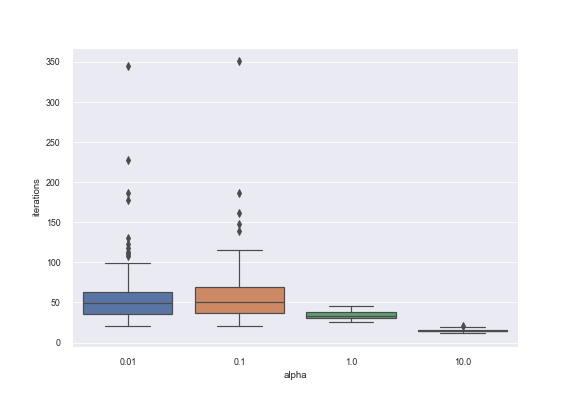
\includegraphics[width=1\linewidth]{images/iterations_boxplot.png}
		\caption{Box plot of number of iterations for each $\alpha$ value}
		\label{fig:boxplot}
	\end{figure}
	
	\begin{table}[ht]
		\centering
		\begin{tabular}{|c||c|c|c|c|}
			\hline
			\textbf{alpha} & 0.01 & 0.1 & 1.0 & 10.0
			\\
			\hline
			\textbf{time} (s) & 23.40 & 22.52 & 13.47 & \textbf{6.09}\\
			\hline
		\end{tabular}
		\caption{Average time to convergence over 100 iterations}
		\label{tab:time}
	\end{table}
	\paragraph{Discussions.} We see that larger values of $\alpha$ results in a smaller time to convergence. This is also seen in Figure~\ref{fig:boxplot} where the distribution of iterations has a smaller, interquartile range and median for larger values of $\alpha$. 
	
	To that end, we observe the Dirchlet distribution over different values of $\alpha$ for $K=3$ in Figure~\ref{fig:alpha}. We observe that the values of $\theta$ are more concentrated given larger $\alpha$. This implies that $\theta$ and from Equation~\ref{eqn:expectation}, $\phi_{ni}$ does not vary much across iterations with larger $\alpha$. As such, convergence happens quickly given that $\phi$ does not change much across iterations and so does $\gamma$.
	
	\begin{figure}
		\centering
		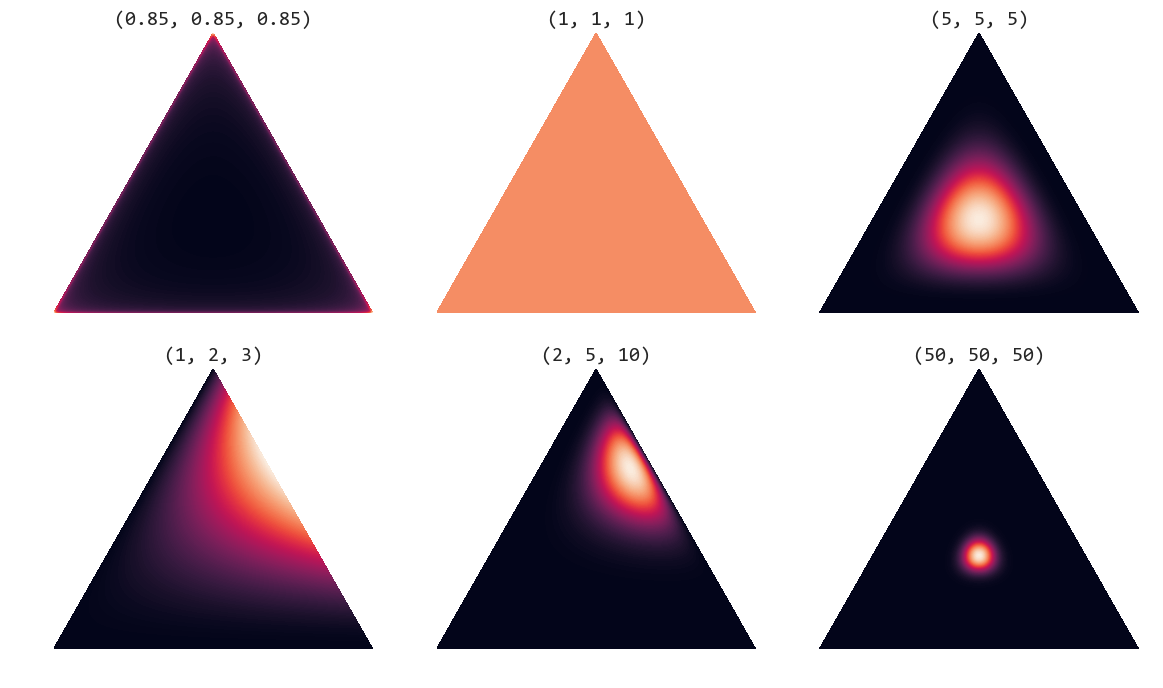
\includegraphics[width=1\linewidth]{images/alpha}
		\caption{Dirchlet Distribution with different values of $\alpha$.}
		\label{fig:alpha}
	\end{figure}
	
	
	\clearpage
	\bibliography{references.bib}
\end{document}